\chapter{ Category 1 constraint Generator : PC reset and fixed labels.}
\label{ch:c1}
This chapter describes working of first algorithm for constraint generation. All four algorithms are different because of different combination of PC label management scheme and  use of dynamic labels. In this algorithm we are using fixed label. Fixed label denotes that label will not change throughout the program. PC reset denotes that after completion of scope of a particular conditional/iteration body PC reset back to the PC just before the execution of conditional/iteration statement. PC monotonic denotes a scheme in which PC label never lose any information once it acquires, it just grows monotonically. This algorithm is able to capture basic information flows within a program, so this algorithm will certify a large number of programs as secure. Program certified secure by this algorithm does not mean that its fully secure, it certifies secure because of the limitation in detection of information flows in program. Some information flows which are not captured by this algorithm may violate information security.\\
\section{Working}
All four algorithm shares same basic structure for parsing input program. Dynamic analysis can not process all branches in a one go but static analysis process all branches in one run. Algorithms generates constraints for all possible control branches in program.  PC keeps track of variables used in conditional statement and iteration statement. Assignment operation are responsible for information flows so at each occurrence of assignment operation constraints generated with the help of PC label.
\section{Constraint Rules}
\begin{enumerate}
	\item < x := e > generate constraint [$\lambda(e)\oplus\lambda(PC)\le\lambda(x)$] and update PC label\\ $\lambda(PC) = \lambda(e)\oplus\lambda(PC)$ 
	\item < x := e > generate constraint [$\lambda(e)\oplus\lambda(PC)\le\lambda(x)$] and update PC label\\ $\lambda(PC) = \lambda(e)\oplus\lambda(PC)$ 
	\item < if e then c1 else c2>  $\forall  x \in ( modified\_global(\hspace{0.2cm} c1 \hspace{0.2cm}and \hspace{0.2cm} c2) \cup \{PC\} )$ generate constraints [$\lambda(e)\oplus\lambda(PC)\le\lambda(x)$] and update PC label $\lambda(PC) = \lambda(e)\oplus\lambda(PC)$
		
	\item < while e do c > $\forall  x \in ( modified\_global(c) \cup \{PC\} )$ generate constraints [$\lambda(e)\oplus\lambda(PC)\le\lambda(x)$] and update PC label $\lambda(PC) = \lambda(e)\oplus\lambda(PC)$
\end{enumerate}

\begin{figure}
	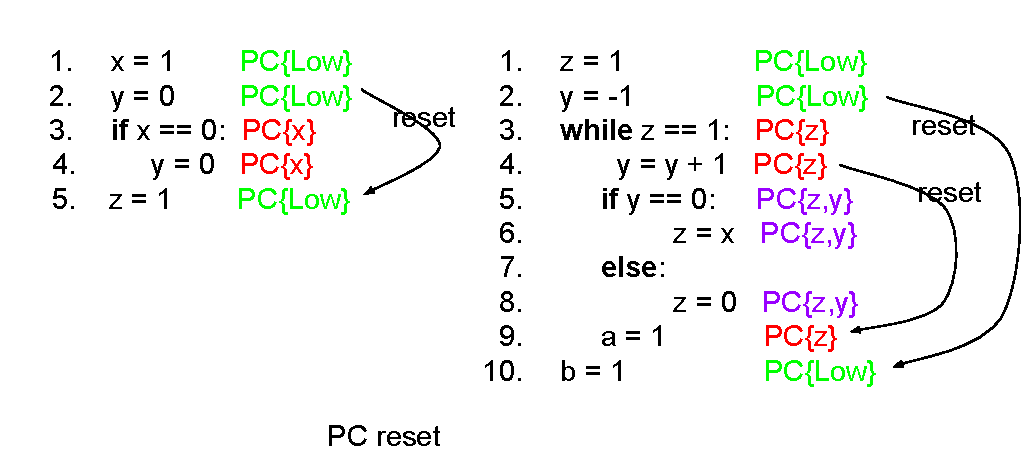
\includegraphics[width=1\textwidth]{PC_reset.pdf}
	\centering
	\caption{Example for PC reset}
	\label{fig:pcreset}
\end{figure}
\begin{figure}
	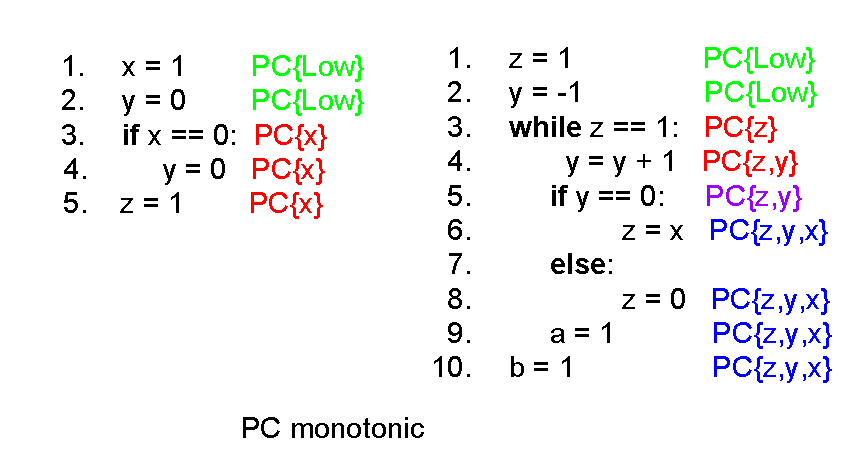
\includegraphics[width=1\textwidth]{PC_monotonic.pdf}
	\centering
	\caption{Example for PC monotonic}
	\label{fig:pcreset}
\end{figure}
\section{Key Idea}
Direct information flow happens because of copying or assigning values. Implicit information flow happens because of control dependency, this algorithm focuses on information flow from variables used in condition statement of if else(conditional)
and while(iteration) to all variables modified in the body of iteration or conditional.
\begin{lstlisting}[language=Python,caption={Python example}, label={lst:p1copy1}]
def(x,y):     #copy x to y
y = 0
z = 0
if x == 0:    # implicit flow x -> z PC{x}
	z = 1
if z == 0:    # implicit flow z-> y PC{z}
	y = 1
p = q         # direct flow q -> p PC{q}
\end{lstlisting}
Constraints generated by this algorithm for listing \ref{lst:p1copy1} are given below. 
\begin{itemize}
	\item x <= z
	\item z <= y
\end{itemize}
\section{Limitations}
For listing \ref{lst:p1copy1} this algorithm is able to capture all information flows, but in more complex programs it may declare falsely a program secure.
\begin{lstlisting}[language=Python, caption=Python version of copy5 example in \cite{denning}. goal: information flow from x to y, label={lst:p1copy5} ]
#Procedure copy5
y = 0
while x==0 :
pass
y = 1
\end{lstlisting}
For listing \ref{lst:p1copy5} this algorithm generated only one constraint Low <= y, that shows this algorithm will certify listing \ref{lst:p1copy5} secure always irrespective of information flow x to y is secure or not. All these limitation in capturing information flow raised because of PC label management in this algorithm is only focus on local information flow. Next algorithm will try to remove these limitation using monotonic PC label management. Appendix A shows the implementation of this algorithm.
\begin{lstlisting}[language=Python, caption=Python version of dynamic label example in \cite{denning}. goal: information flow from x to y, label={lst:p1dynamic} ]
def fun(x, y, z):
a = x
y = a
a = z
fun(x, y, z)
\end{lstlisting}
Another limitation of this algorithm is related to use of fixed label. In listing \ref{lst:p1dynamic} this algorithm detect false information flow z to y. Category 3 uses both dynamic and fixed label to remove this limitation. 